\section{Implementasi Ontologi}
Rancangan ontologi yang telah dijelaskan pada bab sebelumnya akan diimlementasikan pada bab ini. Implementasi rancangan ontologi dilakukan dengan bantuan perangkat lunak Protege versi 5. OWL API versi 4 yang digunakan dalam penelitian ini telah mendukung berbagai macam format serialisasi, salah satu diantaranya adalah Manchester Syntax, oleh karena itu implementasi ketiga ontologi yang akan digunakan pada penelitian ini akan menggunakan Manchester syntax. Manchester syntax dipilih dengan tujuan agar struktur ontologi mudah dipahami.

Implementasi ontologi pariwisata ditunjukkan pada gambar \ref{fig:ntbpar_class}
\begin{figure}[h]
	\centering
	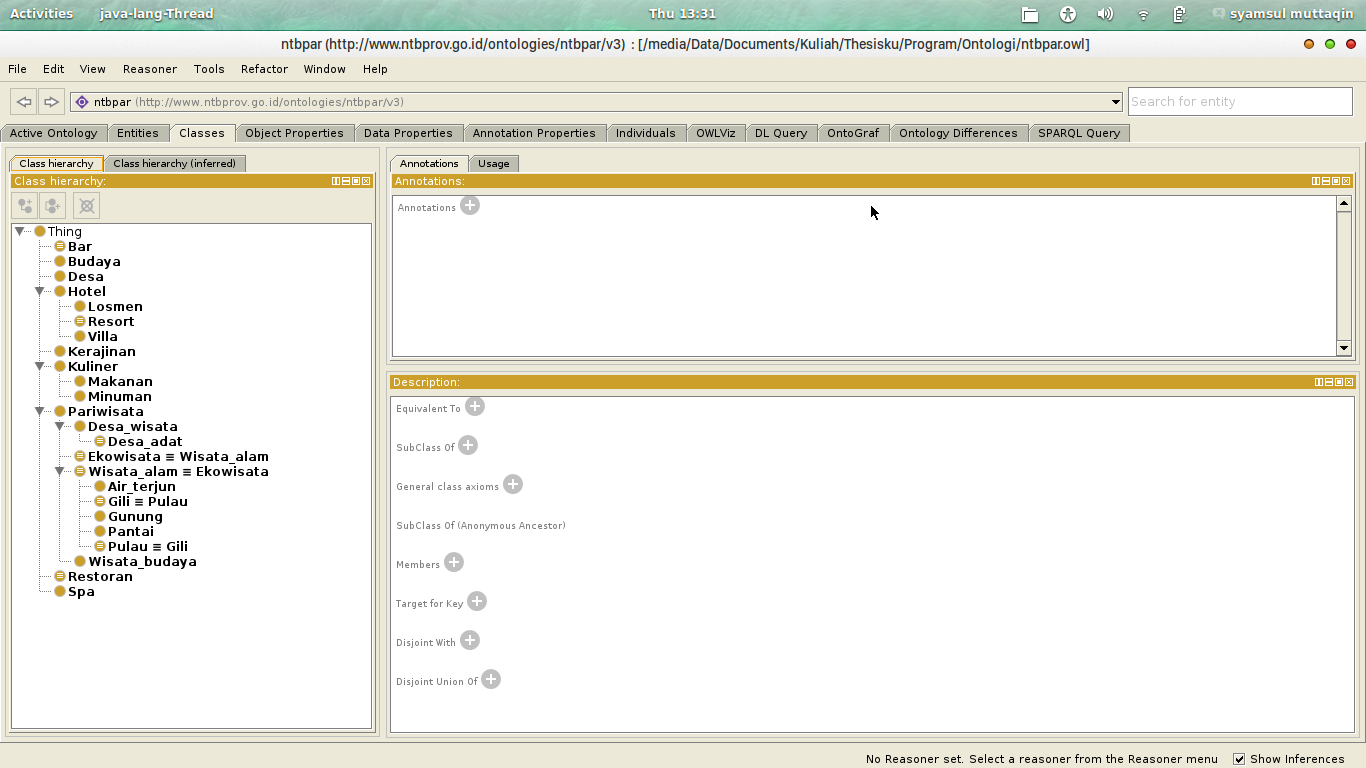
\includegraphics[width=1\textwidth]{ntbpar_class}
	\caption{Implementasi kelas pada ontologi pariwisata}
	\label{fig:ntbpar_class}
\end{figure}

\begin{figure}[h]
	\centering
	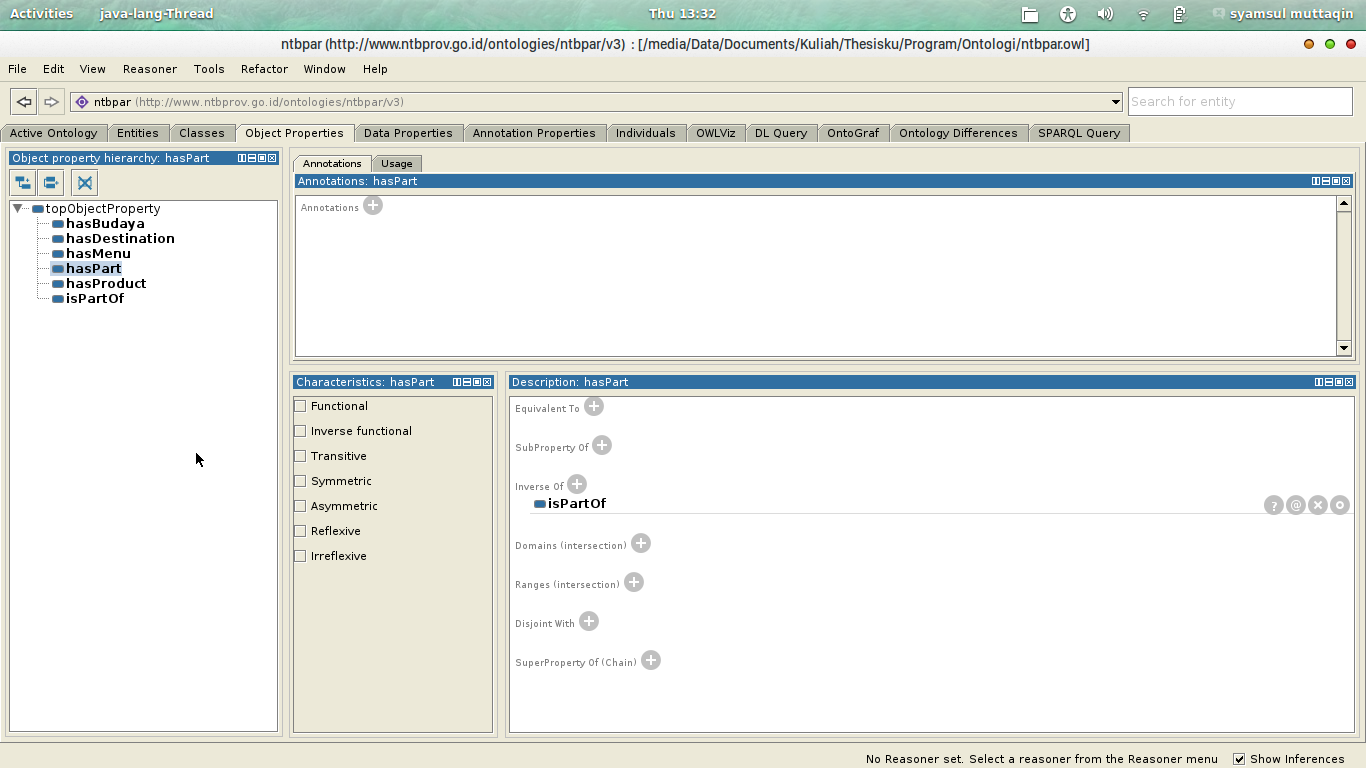
\includegraphics[width=1\textwidth]{ntbpar_op}
	\caption{Implementasi objek properti pada ontologi pariwisata}
	\label{fig:ntbpar_op}
\end{figure}

\begin{figure}[h]
	\centering
	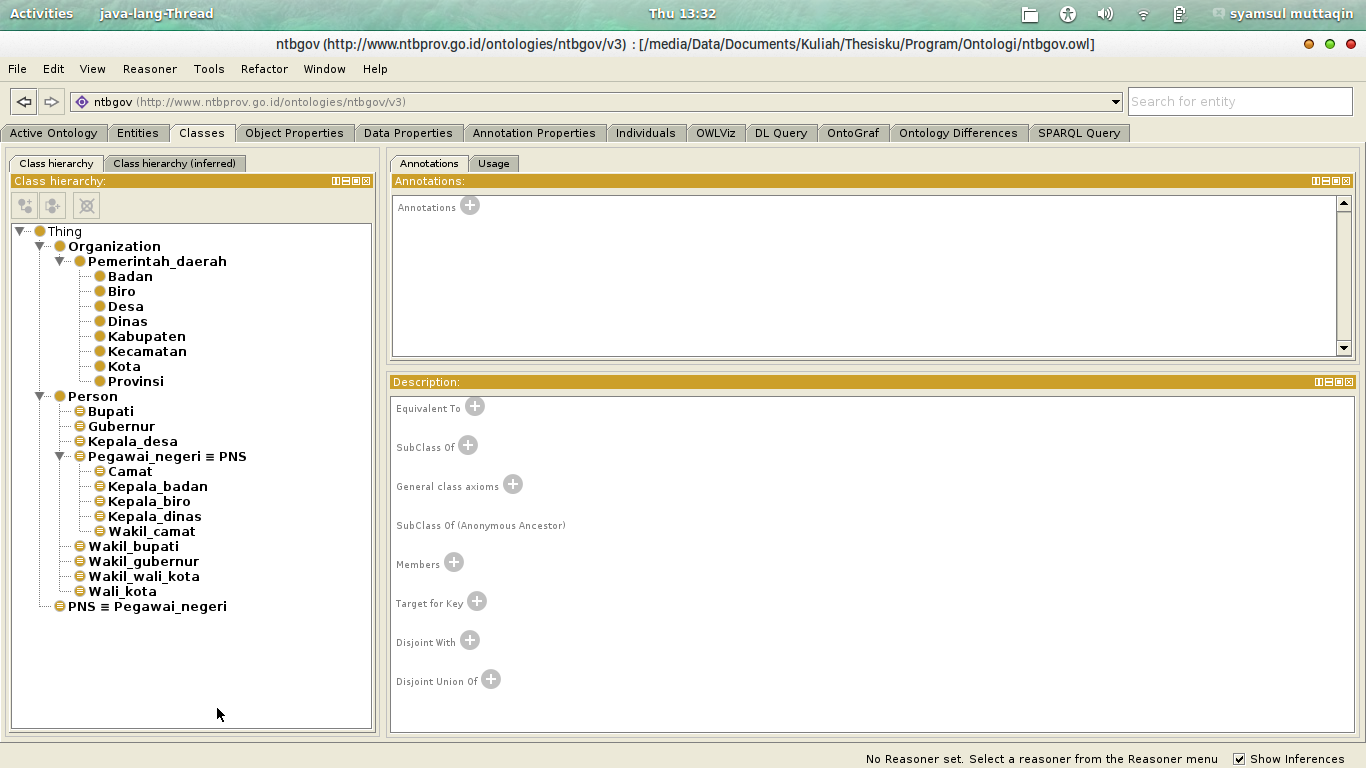
\includegraphics[width=1\textwidth]{ntbgov_class}
	\caption{Implementasi kelas pada ontologi pemerintahan}
	\label{fig:ntbgov_class}
\end{figure}

\begin{figure}[h]
	\centering
	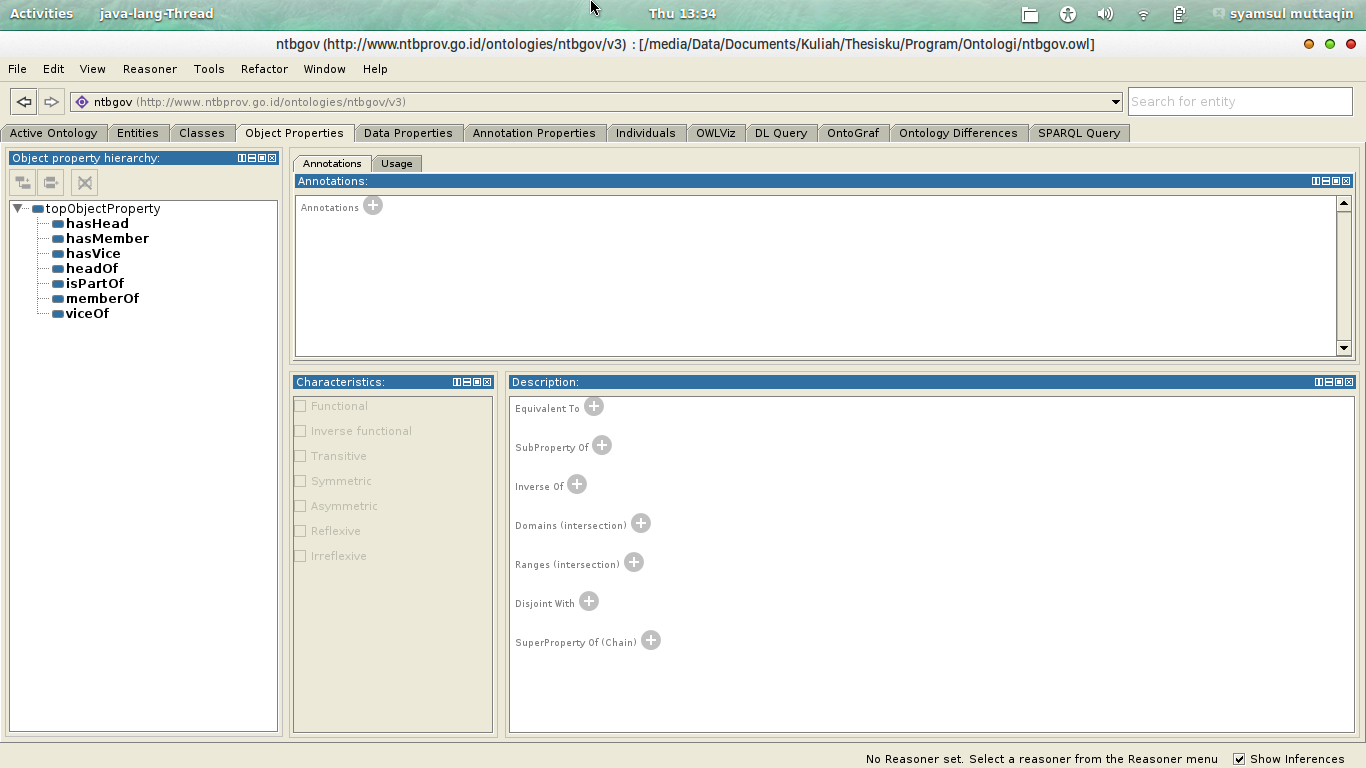
\includegraphics[width=1\textwidth]{ntbgov_op}
	\caption{Implementasi objek properti pada ontologi pemerintahan}
	\label{fig:ntbgov_op}
\end{figure}

\begin{figure}[h]
	\centering
	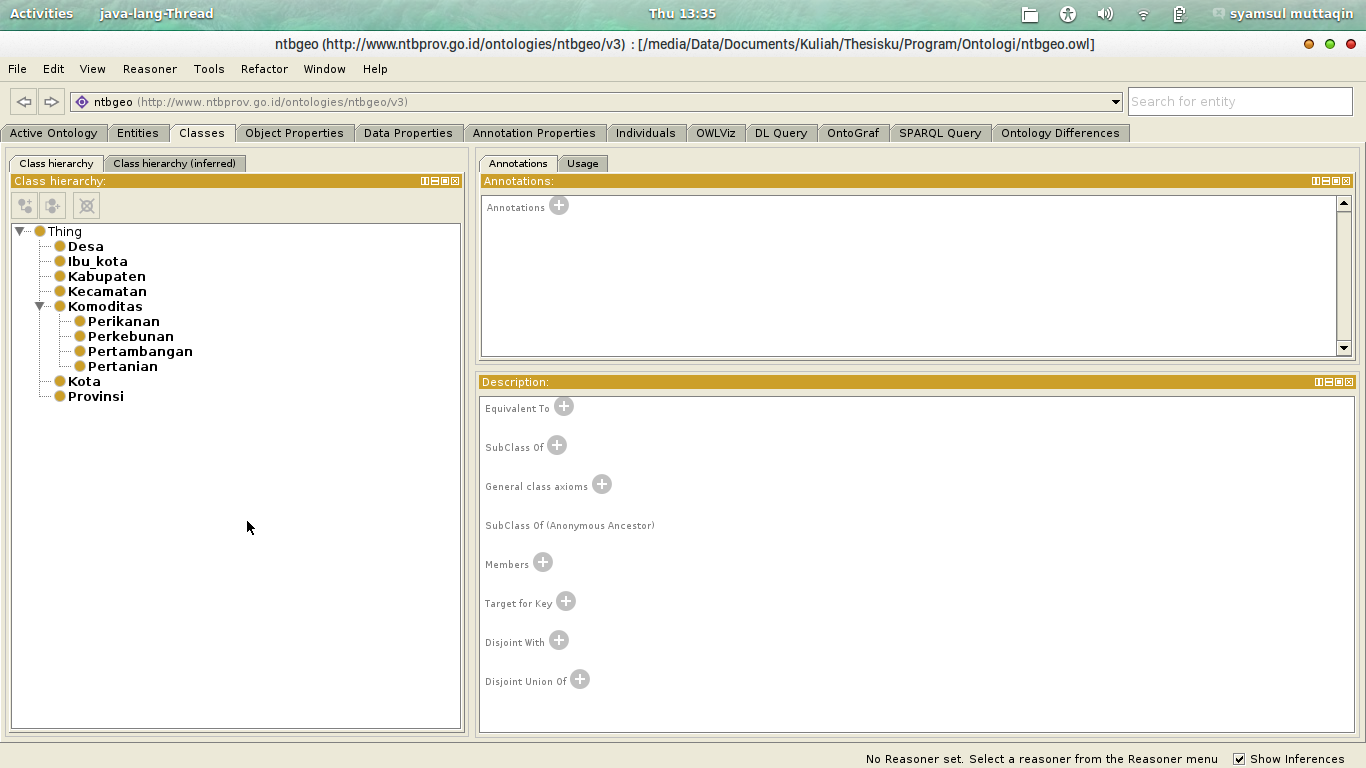
\includegraphics[width=1\textwidth]{ntbgeo_class}
	\caption{Implementasi kelas pada ontologi geografi}
	\label{fig:ntbgeo_class}
\end{figure}

\begin{figure}[h]
	\centering
	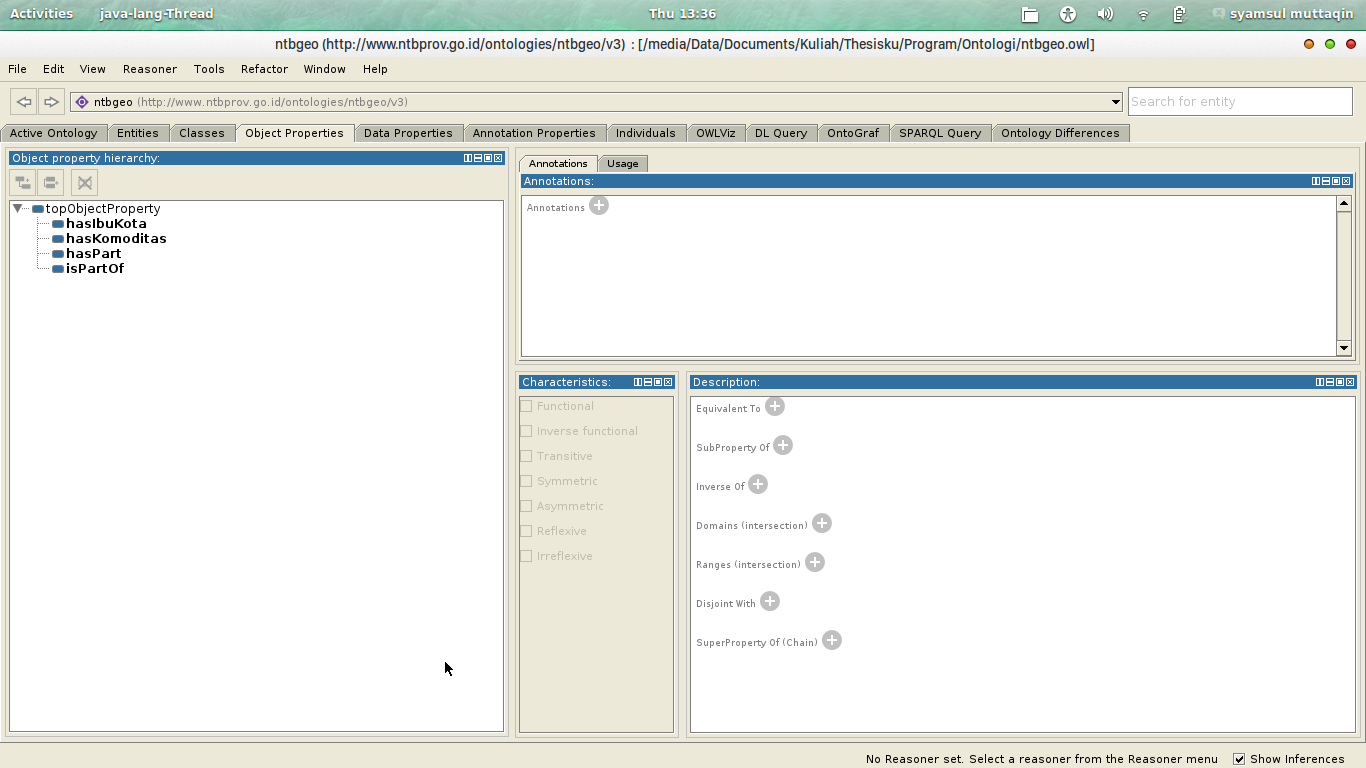
\includegraphics[width=1\textwidth]{ntbgeo_op}
	\caption{Implementasi objek properti pada ontologi geografi}
	\label{fig:ntbgov_op}
\end{figure}

\begin{landscape}
\begin{figure}[h]
	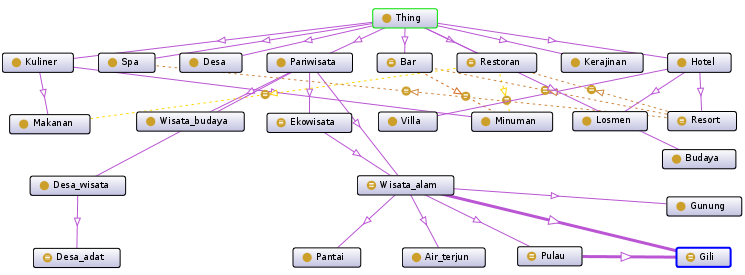
\includegraphics[scale=0.8]{ntbpar}
	\caption{Struktur ontologi pariwisata}
	\label{fig:struktur_ntbpar}
\end{figure}
\end{landscape}

\begin{figure}[h]
	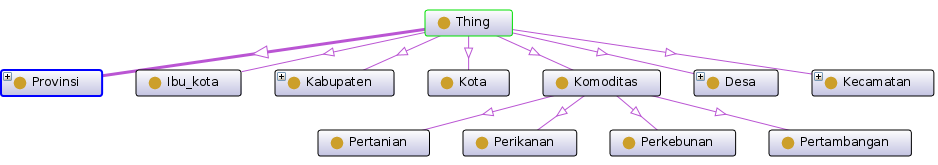
\includegraphics[width=\textwidth]{ntbgeo}
	\caption{Struktur ontologi geografi}
	\label{fig:struktur_ntbgeo}
\end{figure}

\begin{landscape}
	\begin{figure}[h]
		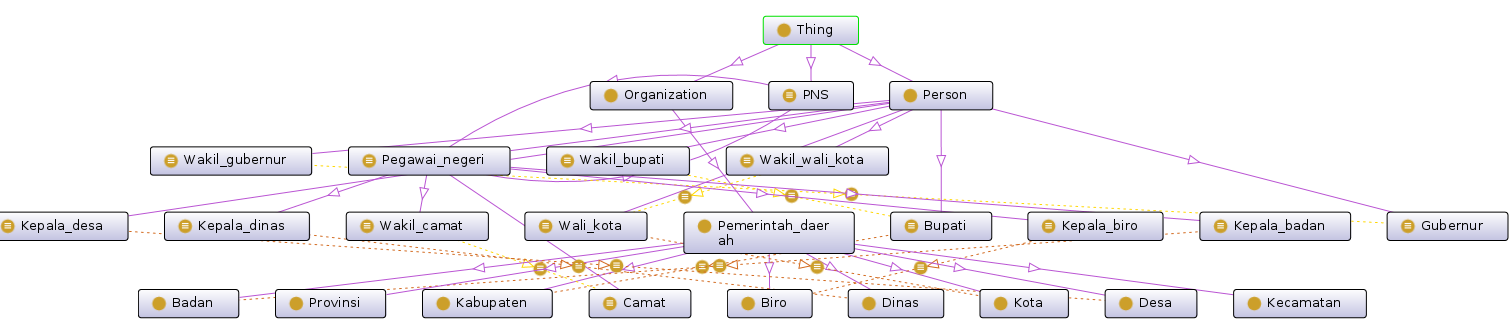
\includegraphics[scale=0.45]{ntbgov}
		\caption{Struktur ontologi pemerintahan}
		\label{fig:struktur_ntbgov}
	\end{figure}
\end{landscape}